\section{Stati Coerenti}
Uno stato coerente fornisce una descrizione classica della luce in termini di onde elettromagnetiche, nonstante siano stati costruiti a partire dalla meccanica quantistica. Viene comunemente rappresentato $|\alpha_j \rangle = |q_j + ip_j \rangle $ attraverso la notazione introdotta da Paul Dirac che prende il nome di \textit{bra-ket}. Come si pu\`o notare uno stato coerente presenta due componenti \textit{q} e \textit{p} dette componenti di quadratura le quali non hanno una valore esatto ma sono variabili aleatorie che rispondono alla stessa distribuzione di probabilit\`a gaussiana che, in oppurtune unit\`a di misura, ha varianza unitaria. Il motivo per cui non rappresentano un valore esatto \`e perch\'e, a differenza fisica classica, nel fisica quantistica le quantit\'a, anche scalari, sono degli operatori che assumono una valore esatto solamente in fase di misura.

Ogni stato coerente presenta un numero medio di fotoni che pu\`o essere calcolato nel seguente modo:
\begin{equation}
\langle n_j \rangle = |a_j|^2 = q^2 + p^2 
\end{equation}

Il numero medio di fotoni di uno stato coerente \`e associato all'energia del segnale di luce che viene inviato, maggiore \`e il numero di fotoni maggiore \`e l'energia del segnale.

Come detto precedentemente, nel nostro caso gli stati coerenti si presentano come una distribuzione di probabilit\`a gaussiana e possono essere rappresentati graficamento nel piano di Gauss come una nuvola di punti i quali avranno appunto probabilit\`a gaussiana di essere estratti.


\begin{figure}[ht] 
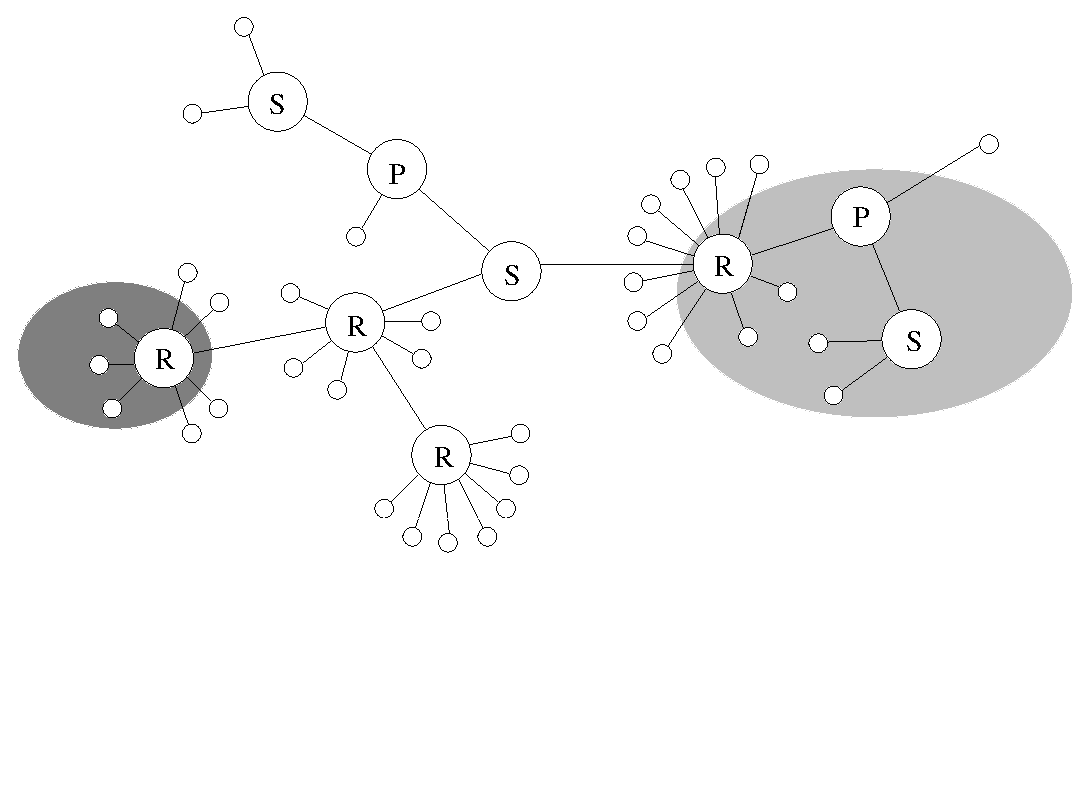
\includegraphics[scale=0.5]{figure/esempio-figura-1.eps}
\caption{Figura da inserire---> Stato coerente} \label{fig:stato-coerente}
\end{figure}

\section{Cosa succede in fase di misura}
In fase di misura Bob riceve una stato coerente con la forma vista in figura \ref{fig:stato-coerente}, ci aspettiamo che nel momento della ricezione il valore della deviazione standard delle gaussiane che descrivono lo stato coerente sia aumentato rispetto a quello che avevano in fase di trasmissione. L'aumento di incertezza \`e dovuto al rumore che viene introdotto dal canale di trasmissione, ma di questo parleremo pi\`u nel dettaglio nel capitolo \ref{cap:capitolo_2}.

Una volta ricevuto il segnale quantistico Bob effettua la misura che consiste nell'estrarre, in base al tipo di misura adottato, uno o due valori che corrispondono ad una delle due componenti di quadratura o entrambe, con pobabilit\`a gaussiana. Dopo questa fase di misura termina la porzione quantistica del protocollo ottenendo dati classici su i quali verrano effettuate altro operazioni per ottenere, in caso di successo, una chiave crittografica sicura con la quale codificare messaggi che verranno scambiati su un canale di comunicazione classico.

\begin{figure}[ht] 
\begin{center}
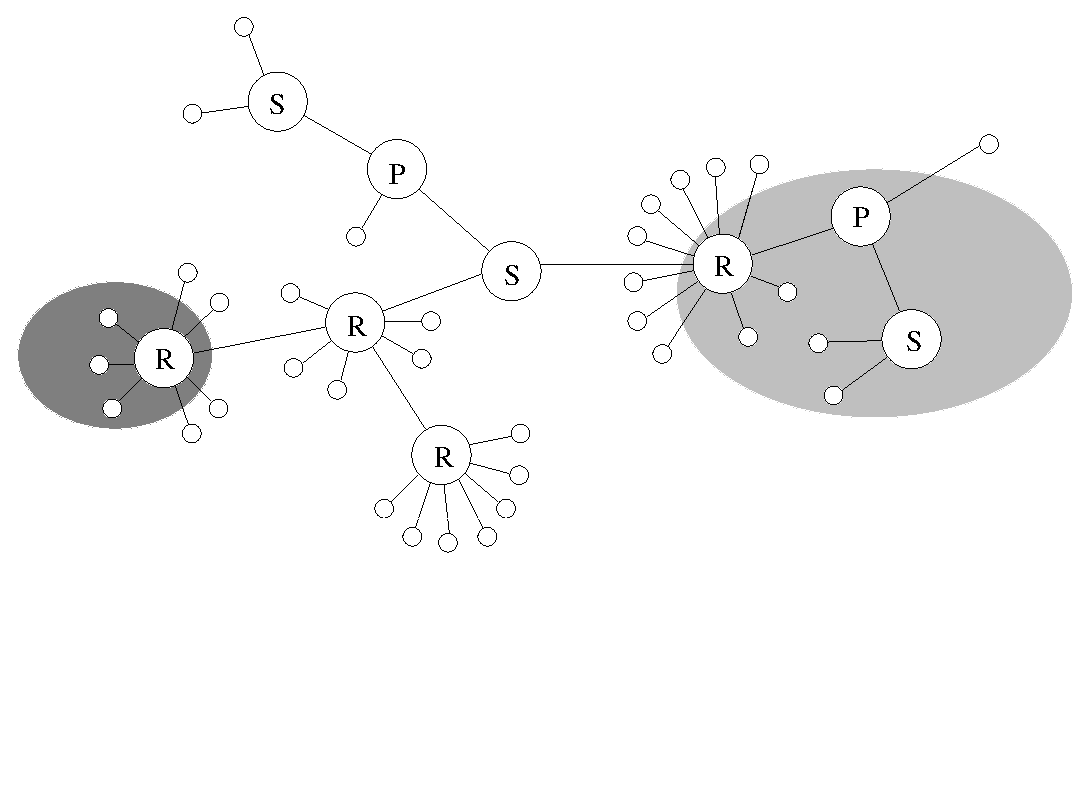
\includegraphics[width=8cm]{figure/esempio-figura-1.eps}
\end{center}
\caption{Figura da inserire---> comparare stato coerente e gaussina dalla quale bob misura} \label{fig:bob-misura}
\end{figure}

